\documentclass[twocolumn]{revtex4}
%\documentclass[onecolumn,12pt]{revtex4}
%\usepackage{amsfonts,amssymb,amsmath,mathbbol}              % for math symbols.
%\usepackage{epstopdf}
%\usepackage{mathbbol}              % for math symbols.
\usepackage{graphics,graphicx,epsfig,ulem} 
\usepackage{amsmath}
\usepackage{multirow}
\usepackage{gensymb}
\usepackage{commath}
\usepackage{textcomp}
\newcommand{\squeezeup}{\vspace{-2.5mm}}

\begin{document}

\textheight=26.385cm
%Change textheight as the last resort...

\title{Determining the viscosity of water} 
 
 
\author{Jacky Cao, Room 205, Thursday, Lab Partners: Peter Dorey, Jon Pritchett \\ Date of experiment: 11/11/2016, Date of report: 20/11/2016}


\begin{abstract}              
 
asdkjasnkdnasd

\end{abstract}

\maketitle

\section{Introduction} 
\vspace{-2ex} 

Derived experimentally by Poiseuille in 1838 and Hagen in 1839 \cite{poiseuillehagen}, the volume flow rate $\frac{dV}{dt}$ of a fluid passing through a tube can be expressed as a function of the density of the fluid $\rho$, the value for acceleration due to gravity $g$, the height the fluid leaves the tube $h$, the radius $a$ and length $L$ of the tube, and the viscosity of the fluid $\eta$,

\begin{equation} 
\frac{dV}{dt}=\frac{\pi}{8}\frac{\rho gh}{\eta}\frac{a^4}{L}. 
\label{pohagen}
\end{equation}

Noting that the group $\rho gh$ can be collectively termed the pressure difference $\Delta P$ between the two ends of the tube \cite{collegephysics}.

If we consider that a fluid is flowing through said tube, it experiences both friction with the inner wall and internal friction within itself. The latter can be defined more readily as the viscosity of the fluid $\eta$, and this results in shear stress when two adjacent layers (laminas) of fluid move relative to each other. 

We find that as $\eta$ increases, the volume flow rate decreases, the shear stress between two laminas becomes greater and so restricts the movement of the fluid's molecules trying to flow through the tube. 

Generally we can say that the lamina flow streamlines are smooth, top layers sliding over other laminas without the system having any turbulent motion - this condition is required for equation [\ref{pohagen}] to be valid. 

Using the relation derived by Hagen and Poiseuille it is possible to experimentally calculate a value for the viscosity of water, $\eta_{water}$.

\vspace{-3ex}
\section{Method} 
\vspace{-2ex}
A flow of water was created by attaching a capillary tube to a water tank, then filling it up with water from 2cm to 16cm at 2cm intervals, this was measured with the markings on the side of the tank. 

As the water flowed out of the tube, a period of 90s was measured on a digital stopwatch. During this period the water which had flowed out was caught within a beaker which was placed on top of a set of digital scales. This allowed for us to measure the mass of the water which had flowed out, and using a pipet and a measuring cylinder we could measure the volume as well.  [BETTER EXPLAIN THIS PART] \\

Three total sets of data were taken for three capillary tube, each tube varied in the internal diameter. This value for diameter was measured using a vernier scale

\begin{figure}[!h]
\begin{center}
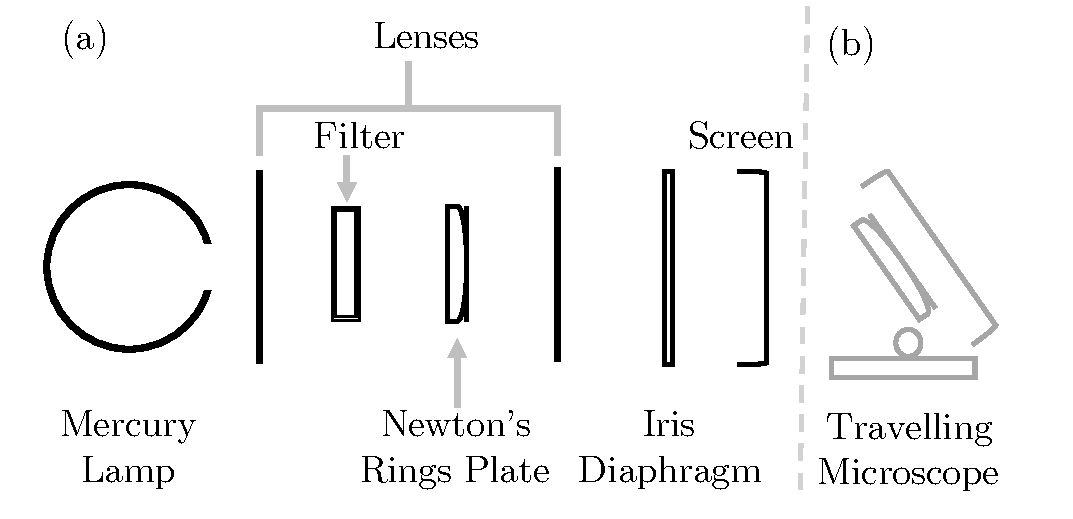
\includegraphics[width=9cm]{fig1}
\caption[]{(a) A schematic of the experimental set-up used to collect the initial set of data. Entire set-up was placed on an optical bench, allowing accurate positioning of the lenses.
\\
(b) Modified set-up used in subsequent investigations - Newton's Rings Plate is moved, the screen is adjusted, and a Travelling Microscope is added.}
\label{fig:fig1}
\end{center}
\end{figure}

askjdnasd

\vspace{-3ex}
\section{Results}
\vspace{-2ex}

asdasd

\vspace{-1ex}
\begin{figure}[!h]
\begin{center}
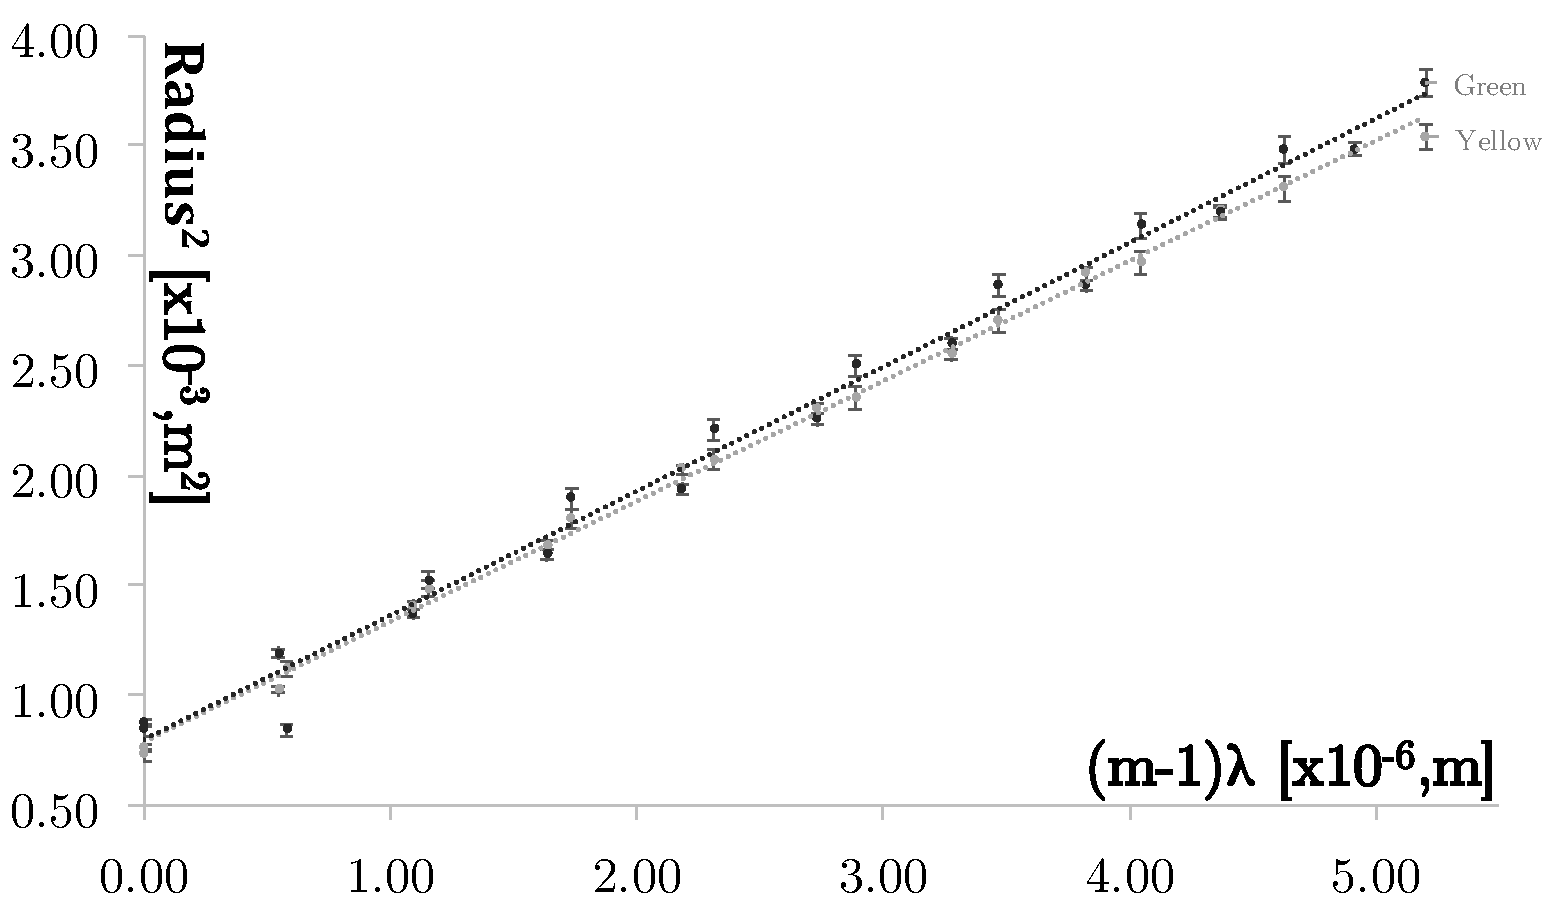
\includegraphics[width=9cm]{fig2}
\caption[]{The fringe radius squared plotted as a function of $(m-1)\lambda$. Horizontal error bars are too small to be seen.}
\label{fig:fig2}
\end{center}
\end{figure}


\begin{table}[h!]
\centering
\begin{tabular}{ |c|c|c|c| } 
 \hline
 \textbf{Experiment} & \textbf{Radius of Curvature, R $[m]$} & $\boldsymbol{d_0} [\times10^{-7}, m]$ \\ [0.5ex] 
 \hline\hline
 $IE$ &$15\pm3$ & $7\pm2$ \\ 
 %$[(m-1)\lambda]_{IE}$ & $R_{IE} = 15\pm3$ & $7\pm2$ \\ 
 %$(m-1)_{IE-Y}$& $16\pm2$ & - \\
 %\hline\hline
 $TM$ & $24\pm2$ & $4.6\pm0.9$ \\
 %$[(m-1)\lambda]_{TM}$ & $R_{TM} = 24\pm2$ & $4.6\pm0.9$ \\
 %$(m-1)_{TM-Y}$ & $21\pm2$ & - \\
 %$(m-1)_{TM-G}$ & $25\pm2$ & - \\
 %$(m-1)_{TM-B}$ & $28\pm1$ & - \\ 
 %\hline\hline
 $RE$ & $18\pm5$ & $8\pm3$ \\
 %$[(m-1)\lambda]_{RE}$ & $R_{RE} = 18\pm5$ & $8\pm3$ \\
 %$(m-1)_{RE-Y}$ & $18\pm3$ & - \\
 %$(m-1)_{RE-G}$ & $19\pm3$ & - \\
 %$(m-1)_{RE-B}$ & $26\pm5$ & - \\
 [1ex] 
 
 \hline
\end{tabular}
\caption{Values for radius of curvature of the planoconvex lens, and their respective values for $d_0$. IE denotes the 'Initial Experiment', TM for 'Travelling Microscope', and RE for 'Repeated Initial Experiment'.}
\label{table:1}
\end{table}

\vspace{-3ex}
\section{Discussion}
\vspace{-2ex}

aksdjnkjasndkjnsakjnd


\vspace{-5ex}
\section{Conclusions}
\vspace{-2ex}
 
askjdnjkasd

\begin{thebibliography}{5}
\bibitem{poiseuillehagen}
	Salvatore P. Sutera and Richard Skalak
	\textit{The History of Poiseuille's Law}.
	Annu. Rev. Fluid Mech., 1993.
	
\bibitem{collegephysics}
	Raymond A. Serway, Chris Vuille, and Jerry S. Faughin
	\textit{College Physics, 8th Edition}.
	Brooks/Cole, Belmont, CA, USA, 2009.

\bibitem{youngandfreedman} 
	Hugh D. Young and Roger A. Freedman.
	\textit{University Physics with Modern Physics, 13th Edition}. 
	Pearson Education Limited, Harlow, Essex, 2015.
	
\end{thebibliography}
\clearpage

\vfill
\twocolumngrid
\vspace{-3ex}
\section*{Appendix}
\vspace{-2ex}

The uncertainty calculated for the radius of curvature $R$ was found by propagating other uncertainties related to quantities found in equation (3). The majority of those uncertainties are calculated using equations based off formulae found in \textit{Measurements and their Uncertainties} [I. G. Hughes and T. P. A. Hase, \textit{Measurements and their Uncertainties}, Oxford University Press, Oxford, United Kingdom, 2010]. 
\\

Firstly for the square of the magnified radius of a bright fringe, $\rho_m^2$, the error is, 
\begin{equation} 
\alpha_{r^2}=\alpha_r\abs{2\times r}
\end{equation}

where $r$ is the value for the magnified radius of a bright fringe, and $\alpha_r$ is it's respective uncertainty. In our experiment this value arises due to a 30 cm ruler being used to measure the diameter, so the highest precision achievable would have been limited at half a division, therefore $\alpha_r$=0.5 cm. 

The uncertainty on the magnification squared, $M^2$, is found by,
\begin{equation} 
\alpha_{M^2}=M^2\abs{2\times\frac{\alpha_M}{M}}
\end{equation}

with $\alpha_{M}$ as the error on the magnification. For the initial and repeated experiment this value was taken to be $0.5$ due to the difficulties in measuring the width of one of the tick-marks with a $30$cm ruler. In the Travelling Microscope experiment $\alpha_{M}=0.005$ due to the precision to which we could measure with the vernier scale.    

To calculate the uncertainty on the radius of curvature $R$, the following equation is thus used,
\begin{equation} 
\alpha_R=R\times\sqrt{\Big(\frac{\alpha_n}{n}\Big)^2 + \Big(\frac{\alpha_{M^2}}{M^2}\Big)^2 },
\end{equation}

where the term $n=(m-1)\lambda$, and the uncertainty on that, $\alpha_n$, was found by using a least squares fitting function in the software Microsoft\textregistered \ Excel. $M^2$ is again, the magnification squared with it's uncertainty $\alpha_{M^2}$ found above in equation (5).  

The uncertainty on $d_0$ is found by further propagating the uncertainties found above, the resulting equation is, 

\begin{equation} 
\alpha_{d_0}=d_0\times\sqrt{\Big(\frac{\alpha_c}{c}\Big)^2 + \Big(\frac{\alpha_{M^2}}{M^2}\Big)^2 + \Big(\frac{\alpha_R}{R}\Big)^2}
\end{equation}

where $c$ is the intercept of the least squares fitting, and $\alpha_c$ is it's respective uncertainty.

With the case of the Travelling Microscope there is also the uncertainty on the vernier scale used, we shall take the highest precision it can measure to be $\alpha_{vernier}=0.5$mm.

\clearpage

%\footnotetext{I am not entirely too sure about what I did for (7), it was help from other students and the demonstrator}

\end{document}